%%%%%%%%%%%%%%%%%%%%%%%%%%%%%%%%%%%%%%%%%%%%%%%%%%%%%%%%%%%%%%%%%%%%%%%%
%    INSTITUTE OF PHYSICS PUBLISHING                                   %
%                                                                      %
%   `Preparing an article for publication in an Institute of Physics   %
%    Publishing journal using LaTeX'                                   %
%                                                                      %
%    LaTeX source code `ioplau2e.tex' used to generate `author         %
%    guidelines', the documentation explaining and demonstrating use   %
%    of the Institute of Physics Publishing LaTeX preprint files       %
%    `iopart.cls, iopart12.clo and iopart10.clo'.                      %
%                                                                      %
%    `ioplau2e.tex' itself uses LaTeX with `iopart.cls'                %
%                                                                      %
%%%%%%%%%%%%%%%%%%%%%%%%%%%%%%%%%%
%
%
% First we have a character check
%
% ! exclamation mark    " double quote  
% # hash                ` opening quote (grave)
% & ampersand           ' closing quote (acute)
% $ dollar              % percent       
% ( open parenthesis    ) close paren.  
% - hyphen              = equals sign
% | vertical bar        ~ tilde         
% @ at sign             _ underscore
% { open curly brace    } close curly   
% [ open square         ] close square bracket
% + plus sign           ; semi-colon    
% * asterisk            : colon
% < open angle bracket  > close angle   
% , comma               . full stop
% ? question mark       / forward slash 
% \ backslash           ^ circumflex
%
% ABCDEFGHIJKLMNOPQRSTUVWXYZ 
% abcdefghijklmnopqrstuvwxyz 
% 101734567890
%
%%%%%%%%%%%%%%%%%%%%%%%%%%%%%%%%%%%%%%%%%%%%%%%%%%%%%%%%%%%%%%%%%%%
%
\documentclass[12pt]{iopart}
\usepackage{graphicx}
\usepackage{enumitem}
\usepackage{natbib}
\usepackage{url}
\RequirePackage{lineno}
\usepackage{fancyhdr}
\usepackage[utf8]{inputenc}

%\newcommand{\gguide}{{\it Preparing graphics for IOP Publishing journals}}
%Uncomment next line if AMS fonts required
\usepackage{iopams}  
\begin{document}

%\pagestyle{fancy}
\lhead{Soil dryness and wildfires in the Apalachicola National Forest}
\rhead{\thepage}
\renewcommand{\headrulewidth}{0pt}

%\setpagewiselinenumbers
%\modulolinenumbers[5]
\linenumbers

\title{Soil dryness and its lead relationship to wildfires in the Apalachicola National Forest, Florida, USA}

\author{Zachery T. Law\textsuperscript{1} \& James B. Elsner\textsuperscript{1}}

\address{\textsuperscript{1}Department of Geography, Florida State University, Tallahassee, FL 32306, USA}

\ead{ztl16@fsu.edu}
\vspace{10pt}
\begin{indented}
\item[]April 2022
\end{indented}

\begin{abstract}

Climate models show rainy seasons getting rainier and dry seasons getting drier due to global warming from increasing greenhouse gases but local changes in drying, the understanding of which is important for mitigation efforts, will not necessarily match the global response. Here long-term weather observations from the Weather Service Office in Tallahassee are used to examine soil moisture deficits and to quantify the extent to which these deficits are related to wildfire occurrences in the nearby Apalachicola National Forest (ANF). Results show a 20\% increase in the average rate of wildfires from May through July for every one cm increase in soil moisture deficit during April. The out-of-sample correlation between the observed number and the predicted rate of wildfires is $+$.57. Tracking daily soil moisture deficits prior to the start of the wildfire season provides a real-time update on developing drought conditions that have had an impact on wildfire activity in the ANF during the weeks to months ahead. Further, long-term upward trends in soil dryness are identified with the most pronounced changes occurring during the driest months. Taken together these findings, and assuming a continuation of the chronic drying, indicate a greater future risk of fires in the ANF.%\footnote{This article is currently under review with {\it Environmental Research Letters}}


\end{abstract}
%
% Uncomment for keywords
%\vspace{2pc}
\noindent{\it Keywords}: wildfires, drought index, soil moisture deficit, seasonal prediction, climate change, Florida

% Uncomment for Submitted to journal title message
%\submitto{\JPA}
%
% Uncomment if a separate title page is required
\maketitle
% 
% For two-column output uncomment the next line and choose [10pt] rather than [12pt] in the \documentclass declaration
%\ioptwocol
%

\section{Introduction}

Climate models show rainy seasons getting rainier and dry seasons getting drier due to global warming from increasing greenhouse gas (GHG) concentrations \citep{ChouEtAl2013}. But local changes in precipitation and drying (e.g., \cite{GossEtAl2020}), which are still unresolved in climate models, will not necessarily match the global response. Importantly it is the local changes that must be causally understood to properly focus mitigation efforts against the resulting impacts.

In this study we use local historical observations to examine soil dryness over time and to quantify the extent to which dryness is related to wildfire. We use local observations from the Tallahassee Weather Service Office (WSO), and we relate variation in dryness computed from these observations to the occurrence of seasonal wildfires in the nearby Apalachicola National Forest (ANF). The goals are to describe the seasonality and trends of forest floor dryness in the ANF using long-term weather records from Tallahassee, to describe the seasonality of wildfires and lightning in the ANF, and to quantify the lead relationship between dryness and wildfire occurrences. 

The objectives are to define the amount of soil dryness in the ANF using the Keetch-Byram Drought Index (KBDI) computed using daily rainfall and maximum temperature values \citep{KeetchByram1968} recorded by the Tallahassee WSO and then to use the KBDI to summarize the seasonality of soil (duff and litter layer) dryness (moisture deficit). Records of wildfires and lightning in the area are used to define the fire season. Daily moisture deficits on days leading up to the wildfire season together with the occurrence of wildfires are used to statistically quantify the lead relationship. Long-term trends in soil moisture deficits are also quantified.

The overarching concern in this paper is the relationship between soil moisture deficit and the number of wildfires in the ANF on the seasonal time scale. This concern is addressed by answering the following questions: (1) By how much does the threat of wildfire increase during the fire season with increases in moisture deficit during the dry season? (2) What long-term changes to soil moisture deficits are occurring in the forest? We answer these questions by examining changes in dryness prior to the fire season and by using an index of soil moisture deficit rather than the lack of rainfall to assess the risk of fire. 

The study is important for forest management mitigation efforts \citep{BeckagePlatt2003} as well as for the health and safety of the communities. Lots of resources are required for planning and implementing a prescribed fire. A seasonal forecast highlighting the potential for fires can help manage those resources toward, among other things, limiting the amount of smoke in the city. Smoke from wildfires, particularly particles at 2.5 microns or smaller, has deleterious effects on human respiratory and cardiovascular systems \citep{Black2017}. Moreover, the hazardous co-occurrence of fine particulate matter and near-surface ozone is more common as wildfires and extreme hot weather increase \citep{KalashnikovEtAl2022}. 

The paper is organized as follows. In section 2 we describe the geographic setting of the study. In section 3 we describe the various data and their sources. In section 4 we analyze soil dryness and in section 5 we analyze data on wildfires in the ANF. In section 6 we develop a statistical model to quantify the lead relationship between dryness and wildfire occurrence. In section 7 we quantify long-term changes in dryness and in section 8 we provide a summary and a discussion of the results. All statistics are computed and all figures made using the R programming language and are available online at \url{https://github.com/jelsner/KBDI}.

\section{Study area}

Droughts have a broad spatial extent so climate change impact studies typically examine a collection of records across many locations. Because long, complete, and homogeneous records are often unavailable, analyses tend to be conducted over a limited time period. By focusing the relationship between soil dryness and the occurrence of wildfires within a spatially limited domain, as we do in this study, we are able to consider changes over a longer period of record than is typically the case. Soil dryness is computed daily from observations made in Tallahassee and the occurrence of wildfires are tallied seasonally from observations made within the ANF (Apalachicola National Forest). 

Tallahassee is the capital city of Florida (USA). It is the county seat and only incorporated municipality in Leon County (see Figure~\ref{ANFMap}). It is the largest city in the Florida Big Bend and Florida Panhandle region. The Tallahassee International Airport, where the WSO observations used in this study were taken, is located on the southwest corner of the city. The urban footprint of the city is adjacent to the ANF.
\begin{figure}[t]
\noindent\includegraphics[scale=.45,trim=0in 1in 0in 0in,clip]{ANFMap.pdf}\\
\vspace{0in}
\caption{Location map. The black boundary surrounding the green areas defines the ANF in this study.}
\label{ANFMap}
\end{figure}

The ANF encompasses more than 2500 square kilometers (about the area of Yosemite National Park) containing some of Florida’s largest intact natural areas where fires are a seasonally common occurrence \citep{Ferguson1998}. Because of its location wildfire frequency and severity in the ANF are not influenced by the confounding effects of urbanization, agricultural land, or roadways. 

The ANF is a publicly managed natural area where various proactive and reactive fire suppression resources are employed \citep{James2006}. The landscape is among the largest remaining semi-wild areas of fire-maintained long-leaf pine savanna in the Southeast United States \citep{Trager2018}. The Köppen climate type is humid, subtropical. The area experiences distinct dry periods in March-April and again in October-November. The spring dry season is followed immediately by the summer lightning season making the period from May through July particularly active for forest wildfires. 

The incidence of lightning-sparked fires is largely a climatic and fuels-driven phenomenon \citep{Littell2016}. Climate change impacts both by increasing flammability (the likelihood something will burn) and the availability of dead, dry litter on the landscape to burn. People and lightning are ignitors. The Marshall Fire in Colorado is a recent example of a climate-enabled weather disaster. 

\section{Data}

\subsection{Tallahassee’s official daily high temperature and rainfall amount} 

This study examines soil dryness computed from daily values of temperature and rainfall. The Tallahassee WSO keeps the log of daily high temperature and rainfall amount (among other variables) as part of the Cooperative Observing Program (COOP). The program includes officially documented station histories that adhere to the U.S. National Weather Service (NWS) approval process. Daily weather records by the WSO are part of the Global Historical Climate Network (GHCN) developed to meet the needs of climate analysis and long-term monitoring studies. The GHCN identification for the Tallahassee records is USW00093805. 

We obtained the data for this station from the National Oceanic and Atmospheric Administration's National Centers for Environmental Information (NCEI). The NCEI is responsible for preserving, monitoring, assessing, and providing public access to historical weather data and information. Before May 1, 1988, a maximum temperature thermometer was used to record the highest temperature for each day after which a hygro-thermometer was used. 

\subsection{The ANF polygon boundary}

We obtain a boundary file for the ANF from the U.S. Department of Agriculture Forest Service in the Enterprise Data Warehouse (EDW) as a polygon shapefile. The EDW is a USFS repository of geospatial and tabular USFS data that is current (refreshed regularly) and standardized (formats, etc), and comes from trusted data sources. The polygon boundary file encompasses 2,567 square kilometers. 

\subsection{Wildfires}

We obtain the location and characteristics of wildfires in the ANF from the Fire Program Analysis (FPA) fire-occurrence database (FOD), which includes 2.17 million geo-referenced wildfire records from federal, state, and local fire organizations, representing a total of 165 million acres burned during the 27-year period 1992-2018 in support of the national Fire Program Analysis (FPA) system \citep{Short2020}. The data elements include discovery date, final fire size, and a point location at least as precise as a Public Land Survey System (PLSS) section (1-square mile grid). The data were transformed to conform, when possible, to the data standards of the National Wildfire Coordinating Group (NWCG), including an updated wildfire-cause standard and basic error-checking was performed, and redundant records were identified and removed, to the degree possible \citep{Short2020}. 

\subsection{Daily lightning counts by county}

We obtain daily counts of lightning strikes by county over the period 1986--2013 from the National Centers for Environmental Information. Wildfires require a spark and fuel. In the United States, half of wildfires are initiated by lighting. The other half are caused by humans. Archived historical lightning data is used in this study to help define the fire season in the ANF.  The lightning strikes recorded by the U.S. National Lightning Detection Network (NLDN) are archived as part of the NOAA Severe Weather Data Inventory (SWDI). The NLDN is a commercial lightning detection network operated by Vaisala. 

\subsection{Gridded daily high temperature and rainfall amount} 

We use daily high temperature and rainfall from the daily PRISM dataset examine the extent to which soil dryness, computed using the Tallahassee WSO weather records, represents the soil dryness across the ANF. PRISM is a set of gridded data for the United States based on a weighted regression that accounts for climate regimes associated with orography, coastal proximate, and other factors \citep{Daly2013}. We use the daily grids at 4 km resolution.

\section{Soil dryness}

We start by examining daily accumulated rainfall and high temperatures in the period 1943-2020. There are five days without a rainfall value and one day without a high temperature value over this period. We fill in the missing values with values from the NCEI daily summaries. The annual average rainfall computed over the 78-year period is 156 cm with a variance of 1096 cm$^2$. The year with the most rain was 1964 with 265 cm and the year with the least rain was 1954 with 78.7 cm. Monthly average daily high temperatures and rainfall amounts peak between June and August (Figure \ref{MonthlyRainTemp}). Monthly rainfall indicates a spring (April-May) and fall (October-November) dry season. As we will show, conditions during the spring dry season are important for fire activity in the ANF. 

\begin{figure}[t]
\noindent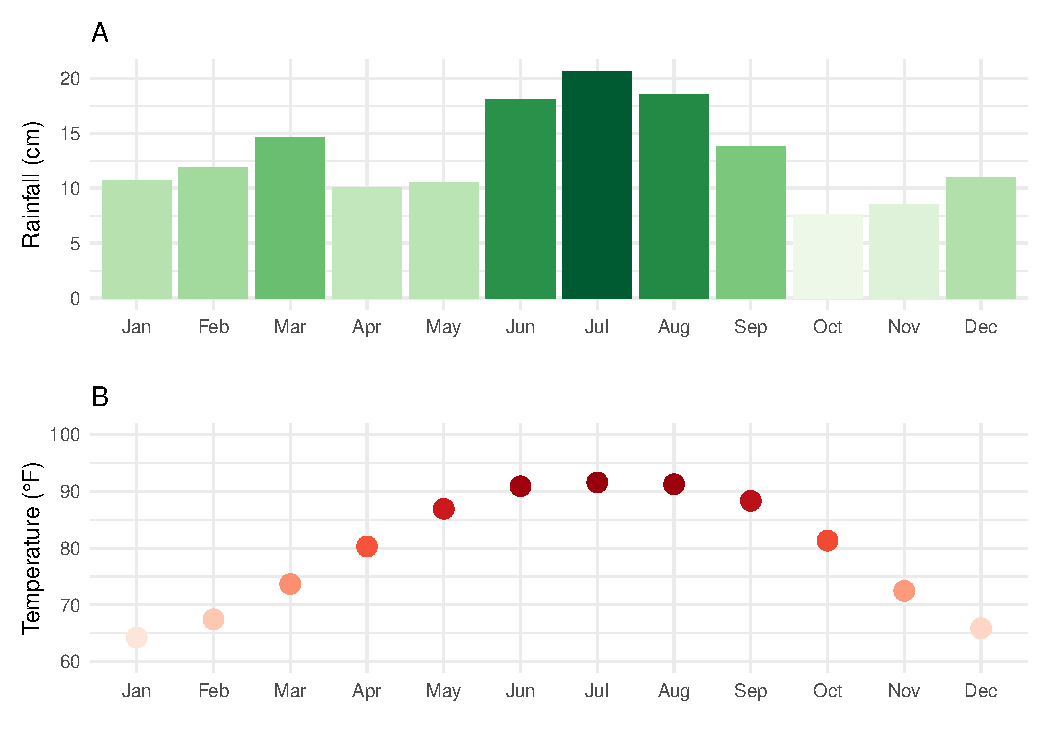
\includegraphics[scale=.8,trim=0in 0in 0in 0in,clip]{MonthlyRainTemp.pdf}\\
\vspace{-.25in}
\caption{Monthly rainfall (A) and average daily high temperature (B) using data from the Tallahassee WSO over the period 1943--2020.}
\label{MonthlyRainTemp}
\end{figure}

From the daily high temperature and rainfall accumulation values we compute the Keetch-Byram Drought Index \citep{KeetchByram1968}. The KBDI assesses the risk of fire by representing the net effect of evapotranspiration and precipitation in producing cumulative moisture deficiency in deep duff and upper soil layers (soil dryness). The index ranges from zero, the point of no moisture deficiency, to 200 mm, the maximum dryness possible. The depth of soil required to hold this amount of moisture varies with soil type; clay = 64 cm, loam = 76 cm, and sand = 203 cm. Prolonged dryness (high values of KBDI) influences fire intensity largely because more fuel is available for combustion (i.e., fuels have a lower moisture content). In addition, the drying of organic material in the soil can make it harder to suppress fires.  

The KBDI relates current and recent weather conditions on the daily timescale to potential or expected fire behavior. It was advanced originally for forest conditions in the Southeast United States and is one of the only drought indexes specifically developed to equate the effects of drought with potential fire behavior \citep{JanisEtAl2002} as opposed to those constructed to monitor hydrological drought \citep{StahlEtAl2020}. \cite{AbatzoglouWilliams2016} found that the correlation coefficient between KBDI and burned area over the forests of southwestern United States ranges between .6 and .8. Direct measurements of soil moisture are now available and can provide slightly better estimates of wildfire risk \citep{KruegerEtAl2017} but there are no long-term records.

Theory under girding the KBDI as a metric for soil moisture deficit (soil dryness) as related to the potential for fires assumes that the vegetation-rainfall relation is close to exponential (determined by evapotranspiration relations) with the rate of moisture removal (transpiring capacity) expressed as a function of the mean annual rainfall. The exponential depletion of moisture starts at a high of 200 mm (saturation) and continues until the wilting point (lowest level) moisture is reached. Details on how to compute KBDI are given in \cite{KeetchByram1968} with a correction made in \cite{Alexander1992}.

Here the KBDI (soil moisture deficit, $D$) is calculated on a daily basis and the values change by $\Delta D$ from one day to the next according to:
\begin{equation}
    \Delta D = (800 - D)\frac{.968 \exp(.0486 T) - 8.3}{1000 \left(1 + 10.88 \exp(-.0441 R)\right)}
\end{equation}
in imperial units where $T$ is the daily maximum temperature (°F); R is the annual accumulated precipitation (in) and $D$ is the KBDI for the previous day. The value of $D$ is reduced by the amount of daily precipitation in excess of .20~in (net rainfall). We convert $D$ in units of hundreds of inches to units of millimeters (SI units) as an estimate of soil moisture deficit. We set the initial value for $D$ on December 31, 1942 at 100 mm. The influence any choice of starting value has on subsequent values of $D$ diminishes to near zero after any saturating rains (typically much less than 60 days). We provide code written in the R Programming Language \citep{RCoreTeam2022} at \url{https://github.com/jelsner/KBDI}.

Daily values of $D$ (soil moisture deficit) are computed from the daily rainfall and temperature over the period 1943--2020 (Figure~\ref{DailyMonthlyDeficits}). Values range between 0 (saturation) and 200~mm (extreme drought). Periods of rainfall and days with lower temperatures contribute to saturated soils while periods without rainfall and days with higher temperatures contribute to soil moisture deficits. Soil drying tends to start in April and continue through June although there is a variation to this pattern depending on the year. There appears to be an expansion of the drying season with more drying occurring in later years.
\begin{figure}[t]
\noindent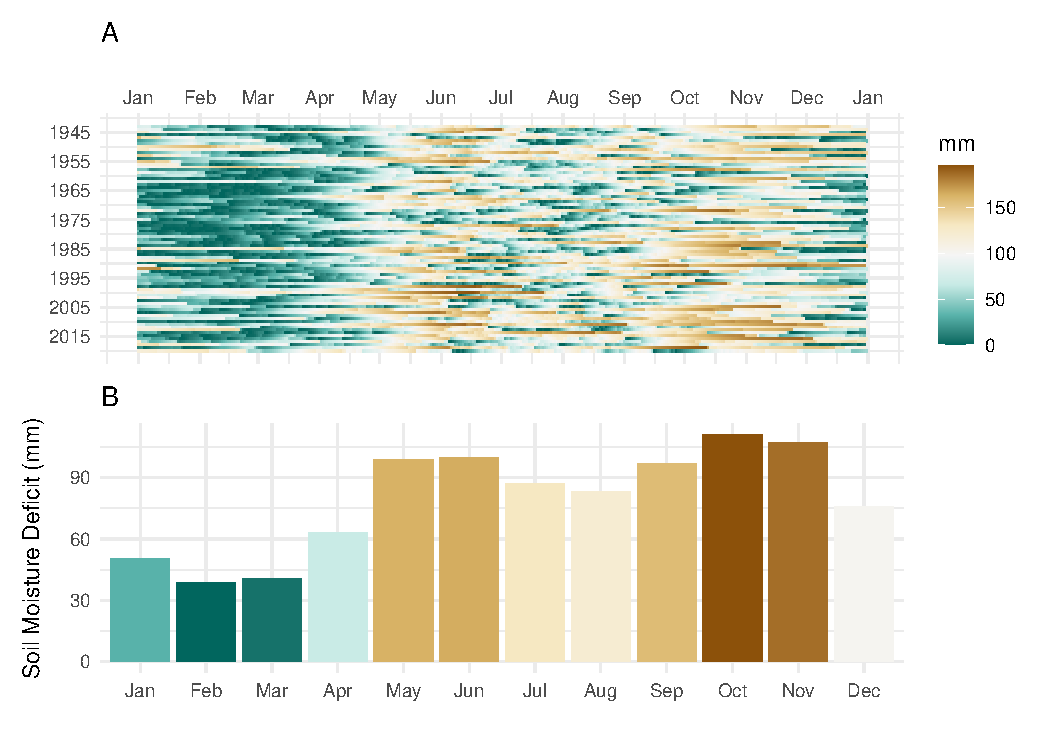
\includegraphics[scale=.85,trim=0in 0in 0in 0in,clip]{DailyMonthlyDeficits.pdf}\\
\vspace{-.25in}
\caption{Daily (A) and monthly (B) soil moisture deficits (mm) estimated using daily rainfall and high temperatures from the Tallahassee WSO over the period 1943--2020.}
\label{DailyMonthlyDeficits}
\end{figure}

The seasonality is highlighted on the monthly time scale with two peaks annually, one during May and June and the other during October and November. Accumulated soil dryness is a combination of the lack of rainfall and evaporation, the latter of which depends on temperature. The spring soil moisture deficit peak occurs as the dry months of April and May get hot during the later half of May into June but before the occurrence of high humidity and thunderstorms during the summer months.

Our interest is soil moisture conditions throughout the ANF, but we use weather data from the nearby Tallahassee WSO to estimate these conditions. This is because we want officially-sited observations over a continuous and lengthy period in order to obtain a quality assessment of long-term changes in these conditions. Here we examine how representative the point estimate of soil moisture conditions is for the ANF as a whole by computing the KBDI across the ANF at 4 km resolution using daily PRISM values of temperature and precipitation (see also \cite{BrownEtAl2021}) over the ten-year period 2009--2018 and then correlating moisture deficits at the grids with the moisture deficits computed from the daily WSO temperature and precipitation values (Figure~\ref{VarianceExplained}).
\begin{figure}[t]
\noindent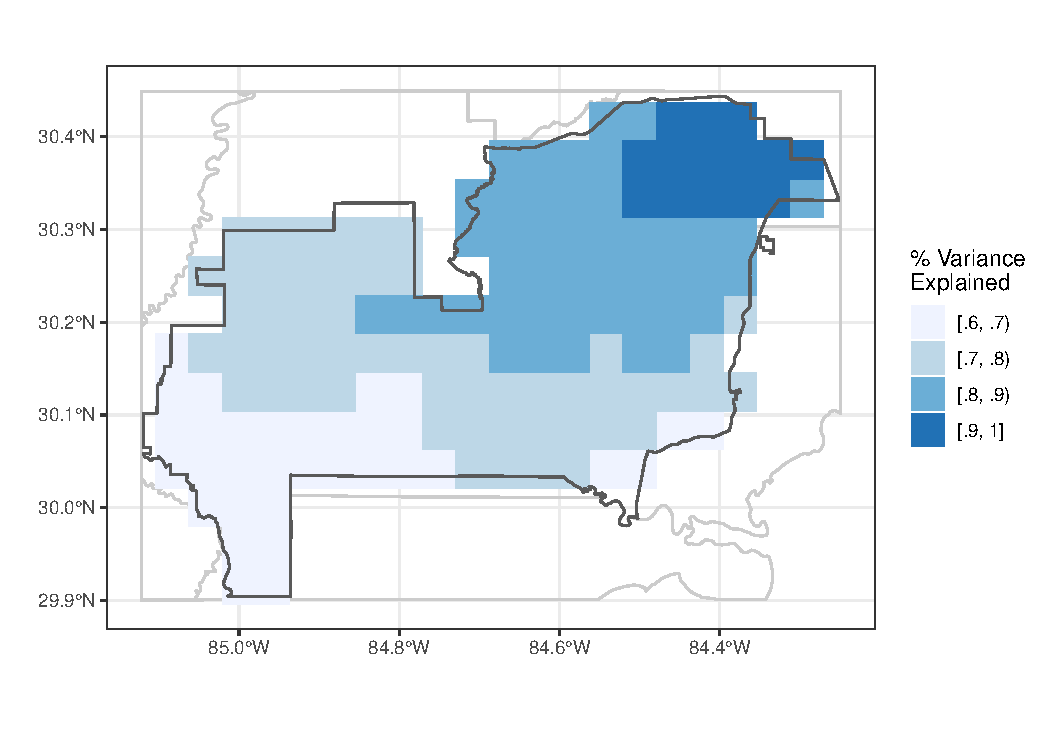
\includegraphics[scale=.8,trim=0in 0in 0in 0in,clip]{VarianceExplained.pdf}\\
\vspace{-.5in}
\caption{The amount of variance explained in moisture deficits computed from the Tallahassee WSO and moisture deficits computed on a 4-km grid using daily values from the PRISM data set.}
\label{VarianceExplained}
\end{figure}

As expected, highest correlations are in the northeast part of the forest closest to the WSO, but the correlations are high throughout the forest. Soil moisture deficits at the Tallahassee WSO explain at least 60\% of the variability in soil moisture deficits at any location in the ANF and more than 80\% of the variability across half of the forest. Importantly, soil moisture deficits computed from the PRISM data should not be used to calculate long-term climate trends due to variations from station equipment and location changes, openings and closings, varying observation times, and the use of short-term networks. In contrast, soil moisture deficits computed at the WSO can be used for analyzing long-term trends.

\section{Wildfires in the ANF}

Natural wildfires caused by lightning account for 40\% of all wildfires in the ANF (Table~\ref{WildfireCauses}). The next leading cause is arson accounting for just over 16\% of all wildfires in the forest. Because of its location, as noted above, wildfire frequency in the ANF is not substantially influenced by the effects of urbanization or roadways. Other causes of fires in the ANF include open burning of debris, recreation and ceremony, vehicles, smoking and power lines. 
\begin{table}[ht]
\centering
\begin{tabular}{rcc}
  \hline
Cause & Number & Percentage \\ 
  \hline
Natural & 437 & 0.40 \\ 
Arson/incendiarism & 181 & 0.16 \\ 
Debris and open burning & 144 & 0.13 \\ 
Missing data/not specified/undetermined & 130 & 0.12 \\ 
Recreation and ceremony &  87 & 0.08 \\ 
Equipment and vehicle use &  44 & 0.04 \\ 
Railroad operations and maintenance &  27 & 0.02 \\ 
Smoking &  25 & 0.02 \\
Power generation/transmission/distribution &  17 & 0.02 \\ 
Misuse of fire by a minor &   7 & 0.01 \\ 
Fireworks &   4 & 0.00 \\ 
Other causes &   2 & 0.00 \\ 
   \hline
\end{tabular}
\caption{\label{WildfireCauses} Causes of wildfires in the ANF.}
\end{table}

There were 437 wildfires for an average spatial intensity of 17 fires per 10 square kilometers over the 27-year period. The spatial distribution of natural fires appears to coincide with an event pattern characterized as complete spatial randomness (Figure~\ref{WildfireLocations}). Indeed, we find only small difference in Ripley’s K functions \citep{Ripley1976}, out to about seven kilometers, computed with distances between fires and computed with distances between events distributed as a Poisson point process, so we fail to reject the null hypothesis of complete spatial randomness.
\begin{figure}[t]
\noindent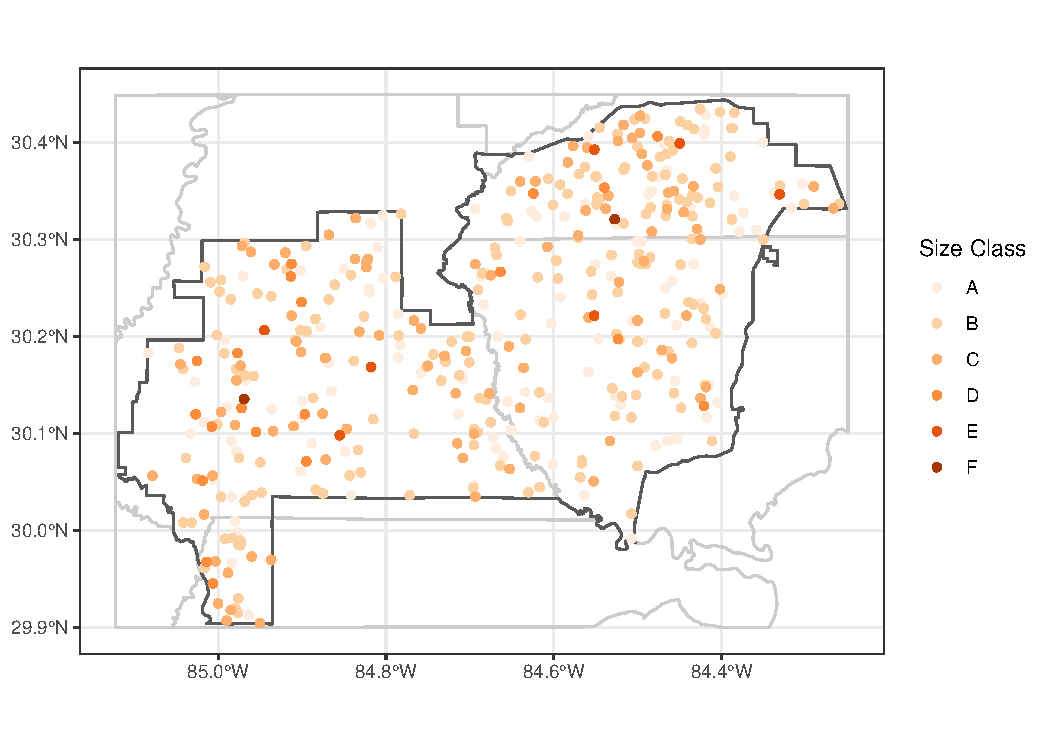
\includegraphics[scale=.8,trim=0in 0in 0in 0in,clip]{WildfireLocations.pdf}\\
\vspace{-.5in}
\caption{Location of natural-caused wildfires in the ANF (1992--2018). Darker color points indicate the fire resulted in a larger burn area.}
\label{WildfireLocations}
\end{figure}

The wildfire season in the ANF is centered on June and includes the months of May and July (Figure~\ref{MonthlyFiresLightning}). More than 80\% of the natural wildfires occur in the three months of May, June, and July. The pronounced peak in June is attributed to the antecedent dry conditions starting in April and the onset of the thunderstorm season which begins in June and peaks in July and August. In fact, cloud-to-ground lightning strikes are most common in the ANF between June through August. Thus, the ANF wildfire season of May through July is a response to the seasonal rhythms of first drying and then thunderstorm activity. In contradistinction the fall dry season is followed by cool-season rainfall without the same threat of lightning so the risk of wildfires is substantially reduced relative to May--July.
\begin{figure}[t]
\noindent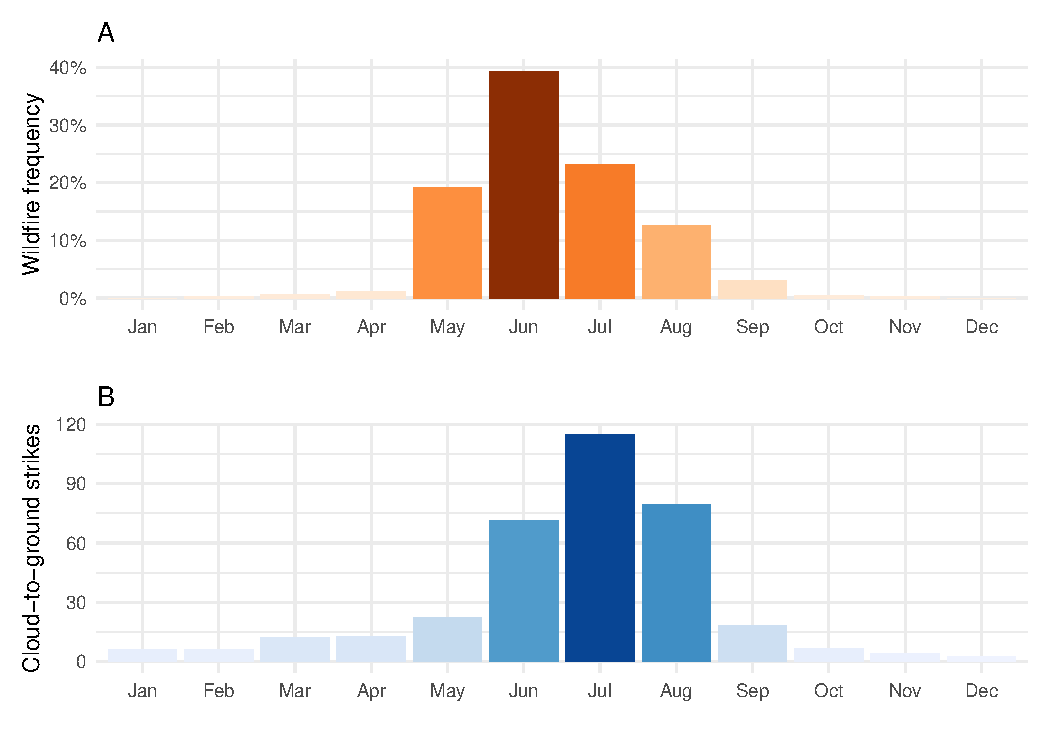
\includegraphics[scale=.8,trim=0in 0in 0in 0in,clip]{MonthlyFiresLightning.pdf}\\
\vspace{-.5in}
\caption{Monthly percentage of natural wildfires (A) and average number of cloud-to-ground lightning strikes in the ANF.}
\label{MonthlyFiresLightning}
\end{figure}

Our objective is to quantify the relationship between the number of wildfires during the wildfire season and dryness occurring prior to the start of the season. The number of wildfires during the wildfire season varies considerably from year to year (Figure~\ref{NumberOfWildfires}). Two years (1997 and 2005) had no fires while 2007 had the most at 49. The average number of fires is 13.2 and the variance is 180. There is no significant correlation between one season and the next (autocorrelation is +.16). But there is a significant correlation [+.44 (+.07, +.70), 95\% confidence interval] between the number of fires and the amount of area burned in a season as expected. Next we explore to what extent can the large interannual variation in the number of wildfires be predicted from soil moisture deficits prior to the start of the season.
\begin{figure}[t]
\noindent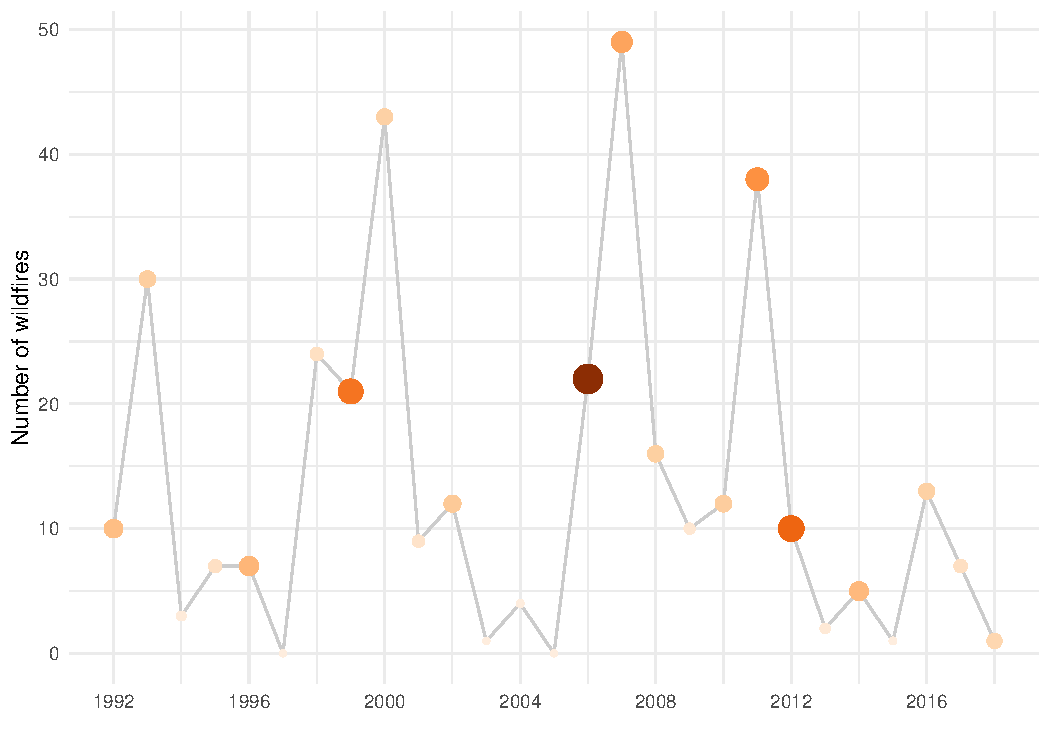
\includegraphics[scale=.8,trim=0in 0in 0in 0in,clip]{NumberOfWildfires.pdf}\\
\vspace{-.5in}
\caption{Seasonal number of natural wildfires in the ANF during May--July. Larger and darker points indicate larger burn area.}
\label{NumberOfWildfires}
\end{figure}

\section{A model for the seasonal number of wildfires}

We begin by examining the bi-variate correlation between the number of wildfires during May--July and soil moisture deficits on days during April. The rank correlation coefficient is $+$.33 at the start of the month and increases to $+$.60 by the end of the month with some fluctuations from day-to-day. In fact the highest correlation of $+$.63 occurs on April 29th. The increase in the strength of the lead relationship between dryness and wildfires is what we would expect since it is the accumulated moisture deficit during the dry season that contributes to the amount of fuel on the forest floor (duff layer) during the wildfire season.

The relationship between soil moisture deficit in April and the number of wildfires during the season is nonlinear with practically no relationship for deficits less than 75 mm (Figure~\ref{Scatterplot}). For increasingly greater soil moisture deficits there is a sharp increase in wildfire occurrence. The 2000 and 2007 wildfire seasons featured the largest number of fires and both ranked in the top five driest.
\begin{figure}[t]
\noindent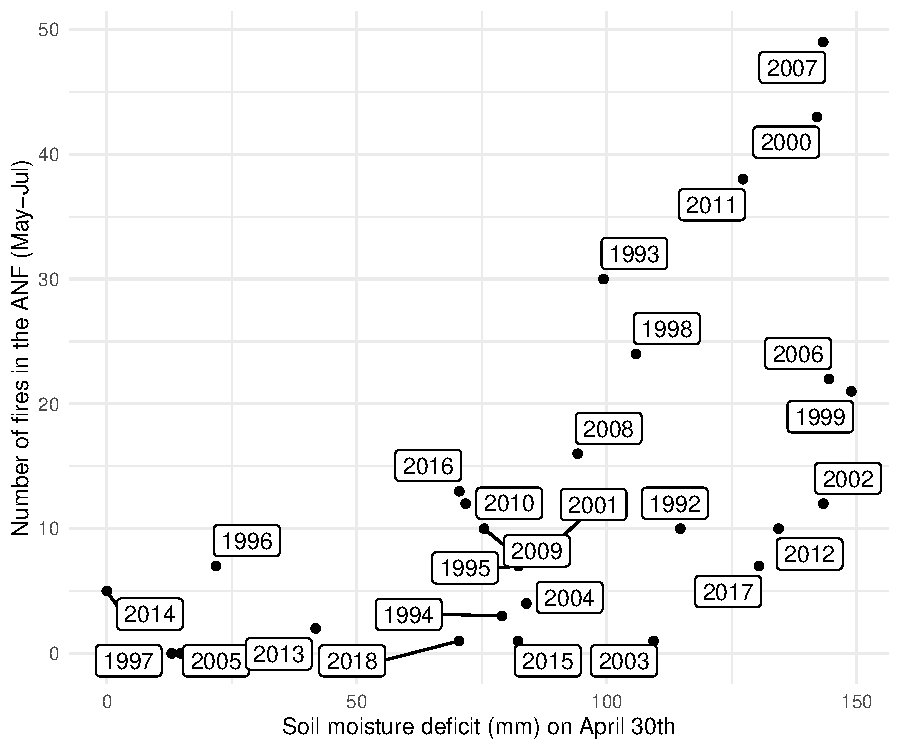
\includegraphics[scale=.8,trim=0in 0in 0in 0in,clip]{Scatterplot.pdf}\\
\vspace{0in}
\caption{Seasonal number of wildfires versus soil moisture deficit (mm).}
\label{Scatterplot}
\end{figure}

To quantify the relationship in terms of wildfire risk per unit change in moisture deficit we use a negative binomial regression model. Negative binomial regression is a generalization of Poisson regression which loosens the restrictive assumption that the variance is equal to the mean made by the Poisson model. Here the ratio of the variance to the mean is 13.6 ($>$ 1). Values for the predictand (number of seasonal wildfires) range between 0 and 49 with a mean of 13.1 fires per fire season. Values for the soil moisture deficit predictor range between 2 cm and 13 cm with an average of 7.3 cm. We re-scale the values to cm to make it easier to interpret the model results.  Since the amount of fuel depends not only on duff layer dryness but also on the amount of duff capable of being burned, we include the previous year's total burn area as a second predictor in the model. Fires remove fuels that diminish the chance of additional fires or limited their spread. Values for the previous burn area range from 135 acres to 34,746 acres with a mean of 4,851 acres.

Mathematically, with the fire season as our fixed exposure window, we fit a negative binomial regression model to the data having the form:
\begin{equation}
    W  \sim \hbox{NegBin}(\hat \mu, n) 
\end{equation}
\begin{equation}
    \ln(\hat \mu) = \beta_0 + \beta_1 D + \beta_2 A \\
%    \ln\left(\frac{P(F)}{1 - P(F)}\right) = \beta_0 + \beta_1 L 
\end{equation} 
\noindent where the seasonal number of wildfires ($W$) is the dependent variable that is assumed to be described by a negative binomial distribution (NegBin) with a rate parameter $\mu$ and a size parameter $n$ \citep{Hilbe2011}. The natural logarithm of the rate parameter is linearly related to soil moisture deficit ($D$) and previous year's burn area ($A$) through the parameters $\beta_0$ (intercept) and $\beta_1$ and $\beta_2$, where $\exp(\beta_1)$ quantifies the relationship between the number of wildfires and the soil moisture deficit as a percentage change in the number of wildfires per cm increase in soil moisture deficit. 

The model is fit using the method of maximum likelihoods carried out in the call to the \texttt{glm.nb} function from \texttt{MASS} package \citep{VenablesRipley2002}. We start by fitting the model having both predictor variables, but find that the previous year's burn area ($A$) does not significantly improve the fit so we remove it before fitting the final model with soil moisture deficit as the sole predictor. We convert soil moisture deficit to units of centimeters (cm) to remove the leading zeros on the coefficients. In the final model, the coefficient estimate on the soil moisture deficit term is $+$.18 with a standard error of .04 (Table~\ref{Coefficients}). This results in a statistically significant term against the null hypothesis that soil moisture deficit in April has no relationship to the seasonal number of wildfires. With a logarithmic link function (Eq.~3) the coefficient is interpret as a 20\% increase in the seasonal rate of wildfires for every 1 cm increase in soil moisture deficit [$1 - \exp(.18) = 20$]. 
\begin{table}[ht]
\centering
\begin{tabular}{rrrrr}
  \hline
 & Estimate & Std. Error & z value & Pr($>$$|$z$|$) \\ 
  \hline
(Intercept) & 0.7368 & 0.4074 & 1.81 & 0.0705 \\ 
  D & $+$0.1767 & 0.0392 & 4.51 & $<$ 0.0001 \\ 
   \hline
\end{tabular}
\caption{\label{Coefficients} Table of coefficients from the negative binomial regression model.}
\end{table}

Model skill is evaluated by comparing the observed wildfire count with the predicted rate from the model. The predicted rate for each season is obtained by plugging the values of the associated explanatory variable into the model. Predicted rates are under dispersed (lower variation) relative to the observed counts. Comparisons are made using the metrics of Pearson correlation coefficient and mean absolute error. Predictive skill using these metrics is evaluated using in-sample and out-of-sample predictions. In-sample predictions are made using all seasons to fit a single model while out-of-sample predictions are made by successively holding one season out of the model fitting procedure and using the particular model to predict the rate from the season left out [hold-one-out cross validation; see \cite{ElsnerSchmertmann1994}]. The out-of-sample predictions give an estimate of how well the model will perform in an operational setting.

The in-sample correlation between the observed number of wildfires and the predicted rate from the model is $+$.65 and the out-of-sample correlation is $+$.57. The in-sample mean absolute error between the observed number of wildfires and the predicted rate from the model is 8.1 wildfires and the out-of-sample mean absolute error is 8.8 wildfires. The in-sample mean squared error is 101 and the out-of-sample mean squared error is 118. The model skill metrics indicate the model has some useful predictive skill. Model precision could be improved with a longer record of wildfire activity.

Predictive uncertainty is assessed through simulations. We first refit the model using a Bayesian framework with a call to the \texttt{brm} function from the \texttt{brms} package \citep{Burkner2021} and then simulate draws from the posterior predictive distribution with calls to functions from the \texttt{tidybayes} package \citep{Kay2022}. The \texttt{brms} package is high level interface to the \texttt{Stan} software \citep{CarpenterEtAl2017}.  A subset of the range of potential model curves together with the observed counts and soil moisture deficits (Figure~\ref{ModelPredictions} shows the uncertainty associated with the expected rate together with the uncertainty associated with a particular count given the expected rate. The spread amongst the model curves is larger for larger counts.
\begin{figure}[t]
\noindent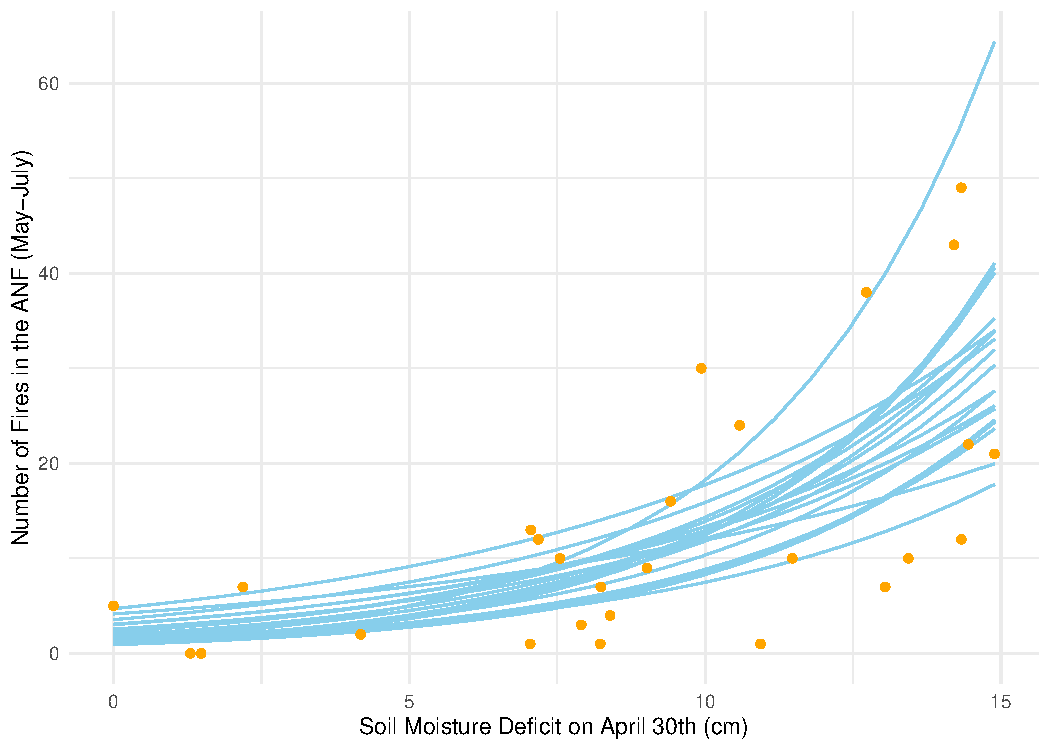
\includegraphics[scale=.8,trim=0in 0in 0in 0in,clip]{ModelPredictions.pdf}\\
\vspace{0in}
\caption{Data values and model curves showing the relationship (observed and predicted) between soil moisture deficit at the end of April and the number of wildfires in the ANF during May through July.}
\label{ModelPredictions}
\end{figure}

\section{Long-term trends in soil moisture deficit}

Having quantified the relationship between soil moisture deficits in April and the frequency of wildfires during May--July, we next quantify long-term trends in dryness. All else being equal, increases in soil moisture deficit during the spring dry season would imply a higher risk of wildfires. Daily soil moisture deficits over the period January 1, 1943 through December 31, 2020 show upward trends in all months with the largest trends noted during the months of April, May, September and October (Figure~\ref{Trends}). 
\begin{figure}[t]
\noindent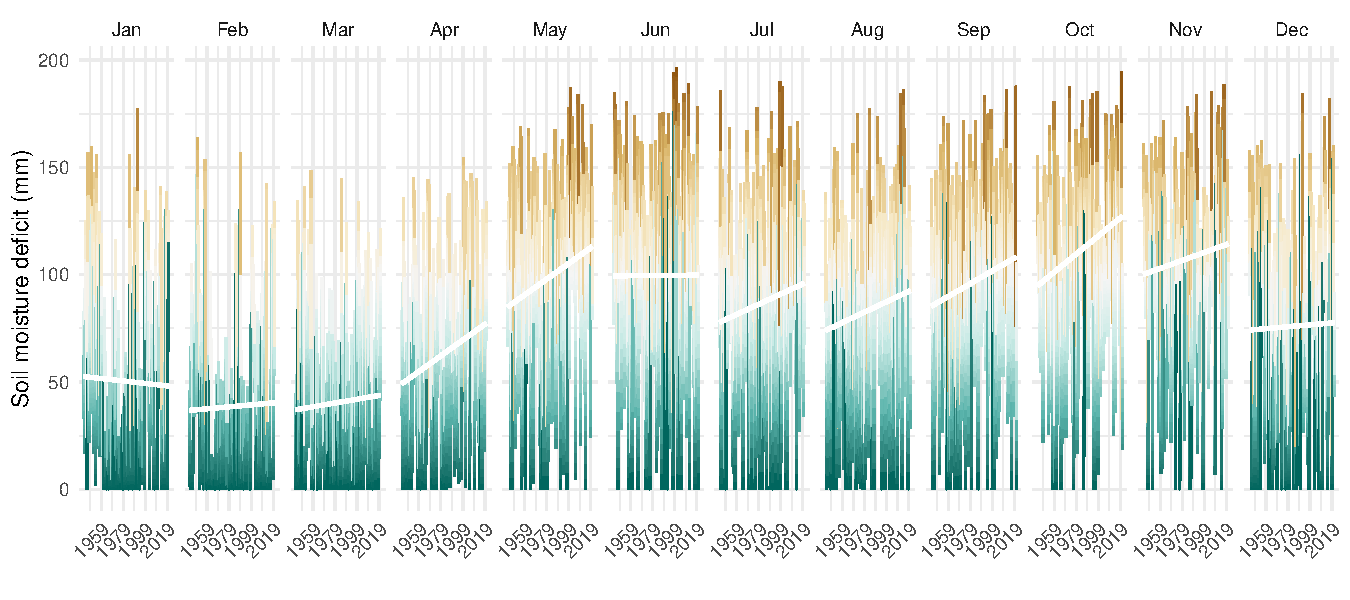
\includegraphics[scale=.67,trim=0in 0in 0in 0in,clip]{Trends.pdf}\\
\vspace{0in}
\caption{Daily soil moisture deficits by day of year. Trend lines are shown in white.}
\label{Trends}
\end{figure}

The Pearson correlation between the monthly trend and monthly dryness is $+$0.5 indicating that upward trends are occurring in months with greatest soil moisture deficits. The upward trend during April, before the wildfire season, amounts to 3.4~mm per decade ($\pm 1.6$~mm/decade, s.e.) and the upward trend during May, at the start of the season, amounts to 2.9~mm per decade ($\pm 1.6$~mm/decade, s.e.). Further we note that fire seasons in the ANF that are drier tend to be hotter because dry days are sunnier.

Another way to quantify the long-term upward trends in soil moisture deficit is to count the the number of days during the year in which the deficit reaches a high value. For example, here we plot the number of days in which soil moisture deficit exceeded 160~mm (Figure~\ref{ExceedanceTrend}). During the 1940s through the 1970s the average number of days at this level of drought was rarely more than 25. Since then nearly half the years have at least this many days of drought.
\begin{figure}[t]
\noindent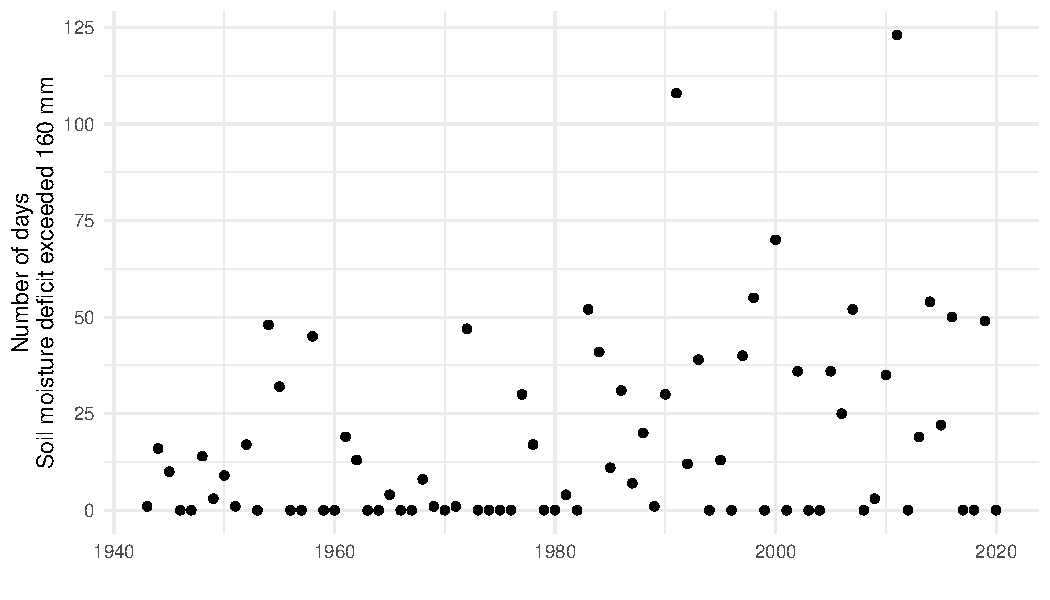
\includegraphics[scale=.8,trim=0in 0in 0in 0in,clip]{ExceedanceTrend.pdf}\\
\vspace{0in}
\caption{Annual number of days in which the soil moisture deficit exceeds 160 mm.}
\label{ExceedanceTrend}
\end{figure}

\section{Summary and discussion}

In this study we used local historical weather observations made by the WSO at the Tallahassee International Airport to examine soil moisture deficits and to quantify the extent to which these deficits are statistically related to wildfire in the ANF. The out-of-sample correlation between the observed number of wildfires and the predicted rate based on soil moisture deficit was $+$.57. We then statistically quantified the long-term upward trends in soil moisture deficits. The main findings indicate (1) a 20\% increase in the average rate of wildfires from May through July for every one cm increase in soil moisture deficit in late April over the period 1992--2018, and (2) an 3.4~mm per decade increase in April soil moisture deficits on average over the period 1943--2020. Taken together these two findings, and assuming a continuation of the drying, indicate a greater future risk of fires in the ANF. 

Large soil moisture deficits create conditions in the forest for the occurrence and spread of wildfires. We demonstrate a strong statistical link between fire frequency and soil moisture deficits prior to the fire season, but soil dryness is not by itself a prerequisite for wildfires. Other weather factors, such as wind and relative humidity play a role in determining the actual fire danger \citep{LiuEtAl2013}. We find no long term changes in wind speed averaged over the fire season. Non-weather factors like prescribed fires also lessen the risk of wildfires \citep{AddingtonEtAl2015}. Our analyses did not include any diagnostics of management intervention but the fact that previous twelve-month burn area is not a significant factor in the prediction model could indicate that current fire management practices are effective in mitigating wildfires. 

Lack of rainfall and high heat can kill trees and dry out the duff and litter layers on the forest floor that act as kindling when a fire sweeps through a forest. Recent research reveals the signature of climate change in the dryness, high heat and longer fire season that can make these fires more frequent and extreme \citep{BrownEtAl2021,GossEtAl2020}. Our findings together with the underlying causal links might have implications for proactively allocating fire suppression resources \citep{KoldenBrown2010,TurcoEtAl2019} in the ANF. Future work will focus on determining to what extent the results generalize to other forests in Florida and the Southeast and on developing a regression model for predicting the amount of forest burned within a season and into a cumulative regression model for predicting fire size class in a manner similar to what we did for predicting the probability of tornadoes by damage category \citep{ElsnerSchroder2019}.

%https://www.who.int/health-topics/wildfires#tab=tab_1 
%https://www.predictiveservices.nifc.gov/outlooks/monthly_seasonal_outlook.pdf 
%https://www.nifc.gov/nicc/predictive/outlooks/outlooks.htm 
%https://www.cpc.ncep.noaa.gov/products/predictions/90day/ 

\section*{Acknowledgements}
This work was supported by the Florida State University.

\section*{Data availability statement}
The data and codes that support the analyzes and findings of this study are openly available from \url{https://github.com/jelsner/KBDI}.

\newpage
\bibliographystyle{agsm}
\bibliography{Wildfire}   % name your BibTeX data base

\end{document}

